\chapter{Analyse des besoins}
\section{Introduction}
Dans ce chapitre, nous allons présenter l'analyse des besoins. En premier lieu, nous parlerons des besoins et des acteurs qui interviennent dans ce projet. Après, nous proposerons un diagramme de cas d'utilisation globale. Ensuite nous présenterons le backlog produit. Et nous clôturons ce chapitre par une exposition de la planification de release.
\section{Capture des besoins}
Le but de notre application est de collecter des informations de l’outil de gestion
de projet Jira\footnote{Jira est un système de suivi de bugs, un système de gestion des incidents, et un système de gestion de projets développé par Atlassian \cite{Jira}.} pour le calcul des indicateurs et de proposer un planning tenant compte de la performance des
équipes. L’application offrira aussi un tableau de bord de suivi des membres de l'équipe (suivi de
performances des membres).
\subsection{Acteurs}
Un acteur est l'idéalisation d'un rôle joué par une personne externe, un processus ou une chose qui interagit avec un système \cite {Acteur}. Les trois acteurs principaux de notre application sont représenté par la figure \ref{code6}.
\begin{figure}[H]
  \centering
  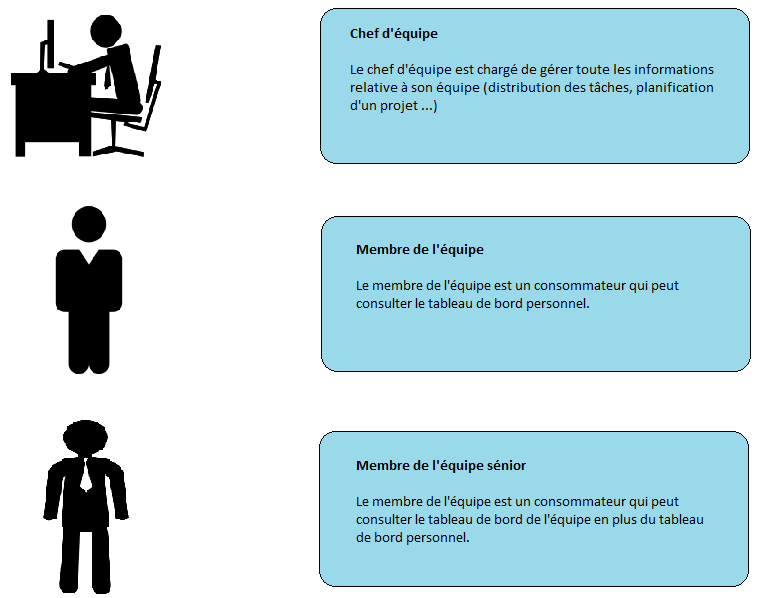
\includegraphics[scale=0.7]{figures/actors.png}
  \caption{Représentation des acteurs}
  \label{code6}
\end{figure}
\subsection{Besoin fonctionnel}
Les besoins fonctionnels représentent ce que le système doit être en mesure d'effectuer. Notre application doit offrir à ces utilisateurs les fonctionnalités suivantes: \\
\begin{itemize}
	\item[$\bullet$] Le membre de l'équipe doit pouvoir:
     \begin{itemize}
     	\item[$\circ$] s'authentifier
        \item[$\circ$] consulter le tableau de bord personnel\\
    \end{itemize}
    \item[$\bullet$] Le membre de l'équipe senior doit pouvoir:
    \begin{itemize}
     	\item[$\circ$] s'authentifier
        \item[$\circ$] consulter les tableaux de bord de l'équipe 
        \item[$\circ$] consulter le tableau de bord personnel\\
    \end{itemize}
	\item[$\bullet$] Le chef d'équipe doit pouvoir:
    \begin{itemize}
    	\item[$\circ$] s'authentifier
        \item[$\circ$] gérer les membres
        \item[$\circ$] gérer les équipes
        \item[$\circ$] consulter les tableaux de bord de l'équipe
        \item[$\circ$] gérer les objectifs des ICP \footnote{Indicateur clé de performance (ICP), en anglais Key Performance Indicator (KPI), est un indicateur mesurable d'aide décisionnelle \cite{ICP}.}
        \item[$\circ$] utiliser la fonctionnalité de planification
     
     
     \end{itemize}
\end{itemize}
\subsection{Besoin non fonctionnel}
Les besoins non fonctionnels peuvent être considérés comme des besoins
fonctionnels spéciaux. Parfois, ils ne sont pas rattachés à un cas d’utilisation
particulier, mais ils caractérisent tout le système (l’architecture, la sécurité, le temps
de réponse, etc.).

Le système doit garantir les besoins opérationnels suivants:\\
\begin{itemize}
	\item[$\bullet$] La sécurité et la confidentialité des données : Les droits d’accès à
l’application doivent être bien attribués aux différents partenaires, afin
d’assurer la sécurité des données.\\
	\item[$\bullet$] Maintenabilité et évolutivité : Le code de l’application doit être bien lisible et
compréhensible pour pouvoir le maintenir facilement et rapidement. En outre,
l’application doit être évolutive afin de répondre aux changements des
besoins fonctionnels.\\
	\item[$\bullet$] Performance: L'application doit garantir un temps de réponse et un temps de traitement réduit.\\
    \item[$\bullet$] Ergonomie: L'application doit avoir une interface conviviale et facile à utiliser et ceci en limitant le nombre des éléments dans l'écran, en utilisant des couleurs qui vont ensemble et en créant des interfaces qui offrent une bonne expérience utilisateur.
\end{itemize}
\section{Diagramme de cas d'utilisation global}
Après avoir identifié les besoins et les acteurs, nous traçons le diagramme de cas d'utilisation global qui sera après la base pour la rédaction du backlog produit.

La figure \ref{code7} présente le diagramme de cas d'utilisation global.
\begin{figure}[H]
  \centering
  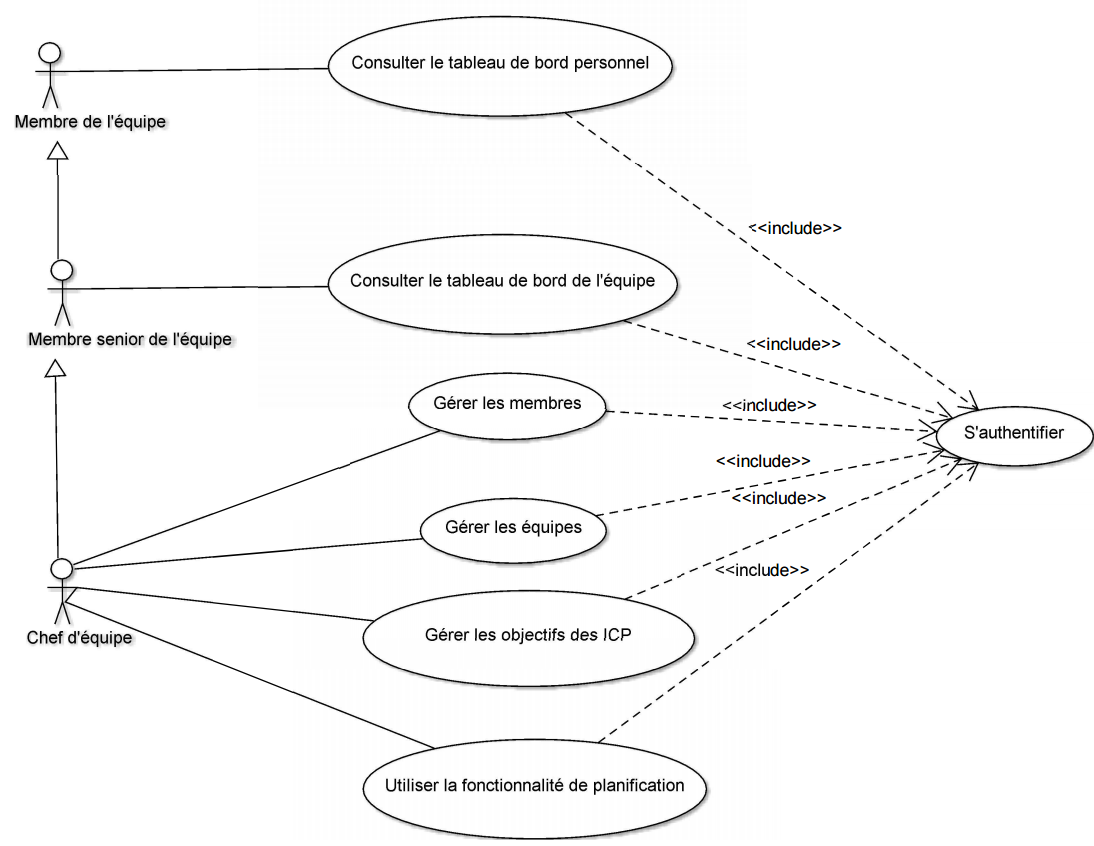
\includegraphics[scale=0.6]{figures/UC_global.png}
  \caption{Diagramme de cas d'utilisation global}
  \label{code7}
\end{figure}
\section{Backlog produit}
Dans Scrum, le backlog produit est la liste des fonctionnalités attendues d'un produit. Il contient donc tous les éléments qui vont nécessiter du travail pour l'équipe. Les éléments y sont classés par priorité ce qui permet de définir l'ordre de réalisation et par complexité ce qui permet de définir la taille d'un backlog sprint.
Nous allons donc présenter les notions de priorité et de complexité. Après nous allons présenter le backlog produit de notre application. Et nous proposerons enfin la planification de release.
\subsection{Notion de priorité}
La priorité représente l'ordre de développement des user stories. Elle permet donc de connaître l'ordre selon lequel les user stories vont être sélectionnées pour être développé dans les backlogs sprint.
Les niveaux de priorité qui vont être utilisé dans notre backlog sont:
\begin{itemize}
	\item[$\bullet$] Élevée: L’exigence est essentielle. Si elle n’est pas faîte le projet échoue.
	\item[$\bullet$] Moyenne: Il s’agit d’une exigence essentielle, qu’il faut faire dans la mesure du possible.
    \item[$\bullet$] Faible: Il s’agit d’une exigence souhaitable. Elle pourrait être faîte dans la mesure où elle n’a pas d’impact sur les autres tâches.
   	\item[$\bullet$] Très faible: Il s’agit d’une exigence "Luxe". Elle ne sera pas faîte cette fois mais plus tard, mais intéressante et à garder pour la prochaine version \cite{Backlog}.
\end{itemize}
\subsection{Notion de complexité}
La notion de complexité(ou Story point) sert à estimer l’effort nécessaire à une équipe pour implémenter une fonctionnalité.
Cette estimation prend en compte l'effort pour le développement, la complexité du développement et le risque \cite{ComplexiteScrum}.

Nous allons utiliser les six premiers nombres de la suite de Fibonacci comme points de complexités dans notre backlog produit (1,2,3,5,8,13) \cite{SuiteFibo}.
\subsection{Backlog produit}
Le tableau \ref{code8} représente le backlog produit de notre application.

\begin{center}
\begin{longtable}{l}
\caption{Backlog produit de l'application} \label{code8} \\
\begin{tabular}{|l|l|l|l|l|l|}
\hline
\textbf{ID} & \textbf{Fonctionnalité} & \textbf{\begin{tabular}[c]{@{}l@{}}ID \\ story\end{tabular}} & \textbf{User Story} & \textbf{Priorité} & \textbf{Complexité} \\ \hline
\multirow{2}{*}{1} & \multirow{2}{*}{s'authentifier} & 1.1 & \begin{tabular}[c]{@{}l@{}}En tant que membre, membre senior \\ ou chef d'équipe, je souhaite pouvoir \\ m'authentifier\end{tabular} & Moyenne & 5 \\ \cline{3-6} 
 &  & 1.2 & \begin{tabular}[c]{@{}l@{}}En tant que membre, membre senior \\ ou chef d'équipe, je souhaite pouvoir \\ modifier mon mot de passe\end{tabular} & Faible & 3 \\ \hline
 
\multirow{3}{*}{2} & \multirow{3}{*}{gérer les équipes} & 2.1 & \begin{tabular}[c]{@{}l@{}}En tant que chef d'équipe, je souhaite \\ pouvoir créer une nouvelle équipe\end{tabular} & Moyenne & 3 \\ \cline{3-6} 
 &  & 2.2 & \begin{tabular}[c]{@{}l@{}}En tant que chef d'équipe, je souhaite \\ pouvoir supprimer une équipe\end{tabular} & Moyenne & 3 \\ \cline{3-6} 
 &  & 2.3 & \begin{tabular}[c]{@{}l@{}}En tant que chef d'équipe, je souhaite \\ pouvoir assigner un chef d'équipe\end{tabular} & Elevé & 3 \\ \hline
 
\multirow{3}{*}{3} & \multirow{3}{*}{gérer les membres} & 3.1 & \begin{tabular}[c]{@{}l@{}}En tant que chef d'équipe, je souhaite\\ pouvoir ajouter un membre dans \\ l'application\end{tabular} & Moyenne & 3 \\ \cline{3-6} 
 &  & 3.2 & \begin{tabular}[c]{@{}l@{}}En tant que chef d'équipe, je souhaite\\ pouvoir supprimer un membre de\\ l'application\end{tabular} & Moyenne & 3 \\ \cline{3-6} 
 &  & 3.3 & \begin{tabular}[c]{@{}l@{}}En tant que chef d'équipe, je souhaite\\ pouvoir modifier un membre de\\ l'application\end{tabular} & Moyenne & 3 \\ \hline
 \end{tabular} \\
 \begin{tabular}{|l|l|l|l|l|l|}
 \hline
 \textbf{ID} & \textbf{Fonctionnalité} & \textbf{\begin{tabular}[c]{@{}l@{}}ID \\ story\end{tabular}} & \textbf{User Story} & \textbf{Priorité} & \textbf{Complexité}
 \\ \hline
4 & \begin{tabular}[c]{@{}l@{}}consulter les \\ tableaux de bord\\ de l'équipe\end{tabular} & 4.1 & \begin{tabular}[c]{@{}l@{}}En tant que membre senior ou chef \\ d'équipe, je souhaite pouvoir consulter \\ le tableaux de bord de l'équipe\end{tabular} & Elevée & 8 \\ \hline
\multirow{2}{*}{5} & \multirow{2}{*}{\begin{tabular}[c]{@{}l@{}}consulter les\\ tableaux de bord\\ personnels\end{tabular}} & 5.1 & \begin{tabular}[c]{@{}l@{}}En tant que membre ou membre senior \\ de l'équipe, je souhaite pouvoir consulter \\ le tableau de bord me représentant\end{tabular} & Faible & 5 \\ \cline{3-6} 
 &  & 5.2 & \begin{tabular}[c]{@{}l@{}}En tant que membre senior ou chef \\ d'équipe, je souhaite pouvoir consulter \\ les tableaux de bord des membres de \\ mon équipe\end{tabular} & Elevée & 13 \\ \hline
6 & \begin{tabular}[c]{@{}l@{}}gérer les objectifs \\ des ICP\end{tabular} & 6.1 & \begin{tabular}[c]{@{}l@{}}En tant que chef d'équipe, je souhaite \\ pouvoir modifier les valeurs des \\ objectifs ICP\end{tabular} & Moyenne & 5 \\ \hline
7 & \begin{tabular}[c]{@{}l@{}}utiliser la \\ fonctionnalité\\ de planification\end{tabular} & 7.1 & \begin{tabular}[c]{@{}l@{}}En tant que chef d'équipe, je souhaite \\ pouvoir saisir les informations relatives \\ à la planification et consulter le résultat \\ obtenu\end{tabular} & Elevée & 13 \\ \hline
\end{tabular}
\end{longtable}
\end{center}

\begin{comment}

\begin{table}[H]
\centering
\caption{Backlog produit de l'application}
\label{code8}
\begin{tabular}{|l|l|l|l|l|l|}
\hline
\textbf{ID} & \textbf{Fonctionnalité} & \textbf{\begin{tabular}[c]{@{}l@{}}ID \\ story\end{tabular}} & \textbf{User Story} & \textbf{Priorité} & \textbf{Complexité} \\ \hline
\multirow{2}{*}{1} & \multirow{2}{*}{s'authentifier} & 1.1 & \begin{tabular}[c]{@{}l@{}}En tant que membre, membre senior \\ ou chef d'équipe, je souhaite pouvoir \\ m'authentifier\end{tabular} & Moyenne & 5 \\ \cline{3-6} 
 &  & 1.2 & \begin{tabular}[c]{@{}l@{}}En tant que membre, membre senior \\ ou chef d'équipe, je souhaite pouvoir \\ modifier mon mot de passe\end{tabular} & Faible & 3 \\ \hline
\multirow{3}{*}{2} & \multirow{3}{*}{gérer les équipes} & 2.1 & \begin{tabular}[c]{@{}l@{}}En tant que chef d'équipe, je souhaite \\ pouvoir créer une nouvelle équipe\end{tabular} & Moyenne & 3 \\ \cline{3-6} 
 &  & 2.2 & \begin{tabular}[c]{@{}l@{}}En tant que chef d'équipe, je souhaite \\ pouvoir supprimer une équipe\end{tabular} & Moyenne & 3 \\ \cline{3-6} 
 &  & 2.3 & \begin{tabular}[c]{@{}l@{}}En tant que chef d'équipe, je souhaite \\ pouvoir assigner un chef d'équipe\end{tabular} & Elevé & 3 \\ \hline
\multirow{3}{*}{3} & \multirow{3}{*}{gérer les membres} & 3.1 & \begin{tabular}[c]{@{}l@{}}En tant que chef d'équipe, je souhaite\\ pouvoir ajouter un membre dans \\ l'application\end{tabular} & Moyenne & 3 \\ \cline{3-6} 
 &  & 3.2 & \begin{tabular}[c]{@{}l@{}}En tant que chef d'équipe, je souhaite\\ pouvoir supprimer un membre de\\ l'application\end{tabular} & Moyenne & 3 \\ \cline{3-6} 
 &  & 3.3 & \begin{tabular}[c]{@{}l@{}}En tant que chef d'équipe, je souhaite\\ pouvoir modifier un membre de\\ l'application\end{tabular} & Moyenne & 3 \\ \hline
4 & \begin{tabular}[c]{@{}l@{}}consulter les \\ tableaux de bord\\ de l'équipe\end{tabular} & 4.1 & \begin{tabular}[c]{@{}l@{}}En tant que membre senior ou chef \\ d'équipe, je souhaite pouvoir consulter \\ le tableaux de bord de l'équipe\end{tabular} & Elevée & 8 \\ \hline
\multirow{2}{*}{5} & \multirow{2}{*}{\begin{tabular}[c]{@{}l@{}}consulter les\\ tableaux de bord\\ personnels\end{tabular}} & 5.1 & \begin{tabular}[c]{@{}l@{}}En tant que membre ou membre senior \\ de l'équipe, je souhaite pouvoir consulter \\ le tableau de bord me représentant\end{tabular} & Faible & 5 \\ \cline{3-6} 
 &  & 5.2 & \begin{tabular}[c]{@{}l@{}}En tant que membre senior ou chef \\ d'équipe, je souhaite pouvoir consulter \\ les tableaux de bord des membres de \\ mon équipe\end{tabular} & Elevée & 13 \\ \hline
6 & \begin{tabular}[c]{@{}l@{}}gérer les objectifs \\ des ICP\end{tabular} & 6.1 & \begin{tabular}[c]{@{}l@{}}En tant que chef d'équipe, je souhaite \\ pouvoir modifier les valeurs des \\ objectifs ICP\end{tabular} & Moyenne & 5 \\ \hline
7 & \begin{tabular}[c]{@{}l@{}}utiliser la \\ fonctionnalité\\ de planification\end{tabular} & 7.1 & \begin{tabular}[c]{@{}l@{}}En tant que chef d'équipe, je souhaite \\ pouvoir saisir les informations relatives \\ à la planification et consulter le résultat \\ obtenu\end{tabular} & Elevée & 13 \\ \hline
\end{tabular}
\end{table}
\end{comment}

\subsection{Prototypage des interfaces}
La figure \ref{code10} présente le prototype de l'interface de la page d'authentification.
\begin{figure}[H]
  \centering
  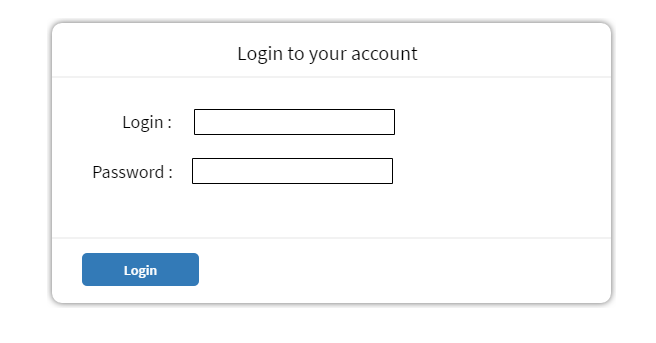
\includegraphics[scale=1]{figures/prototypes/Login_form.PNG}
  \caption{Prototype de la page d'authentification}
  \label{code10}
\end{figure}
La figure \ref{code11} présente le prototype du tableau de bord personnel où nous retrouverons toutes les statistiques concernant l'utilisateur connecté.
\begin{figure}[H]
  \centering
  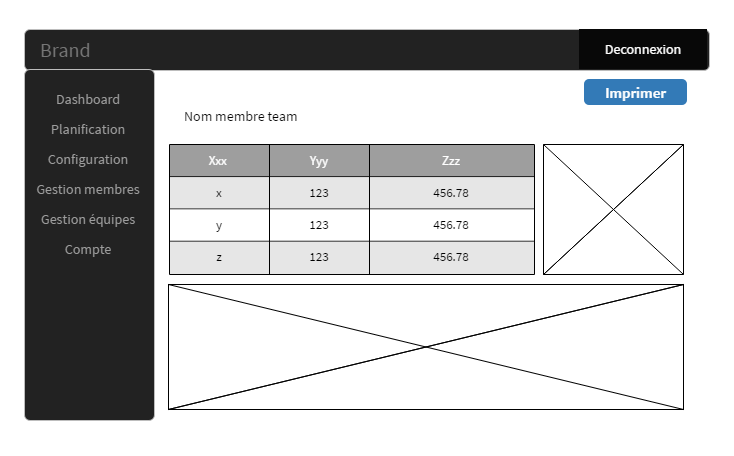
\includegraphics[scale=0.74]{figures/prototypes/Member_dashboard.PNG}
  \caption{Prototype du tableau de bord personnel}
  \label{code11}
\end{figure}
La figure \ref{code12} présente le prototype du tableau de bord de l'équipe ou en retrouve des statistiques qui concernent toute l'équipe.
\begin{figure}[H]
  \centering
  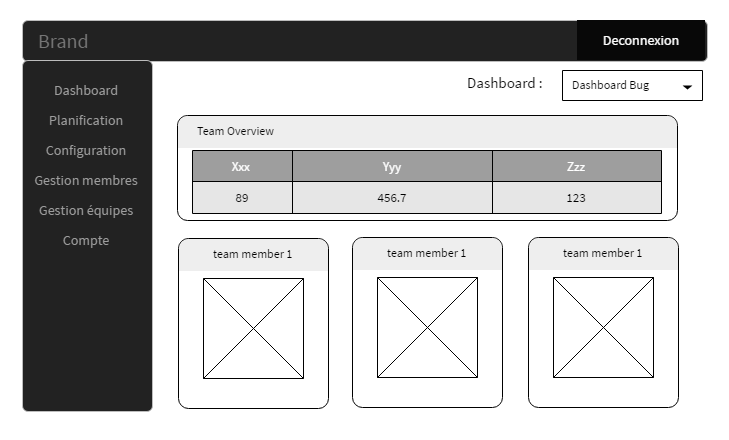
\includegraphics[scale=0.74]{figures/prototypes/Team_dashboard.PNG}
  \caption{Prototype du tableau de bord de l'équipe}
  \label{code12}
\end{figure}
La figure \ref{code13} présente le prototype de l'interface de gestion de compte où l'utilisateur peut changer son mot de passe.
\begin{figure}[H]
  \centering
  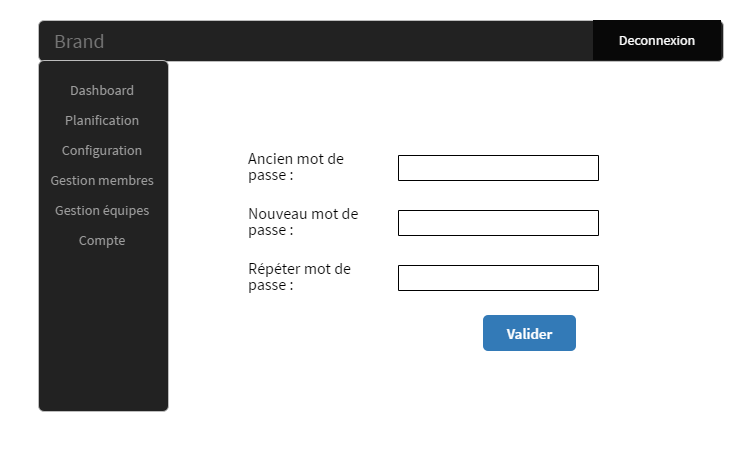
\includegraphics[scale=0.74]{figures/prototypes/Compte.PNG}
  \caption{Prototype de la gestion de compte}
  \label{code13}
\end{figure}
La figure \ref{code14} présente le prototype de l'interface de gestion des objectifs ICP ou l'utilisateur peut modifier les objectifs.
\begin{figure}[H]
  \centering
  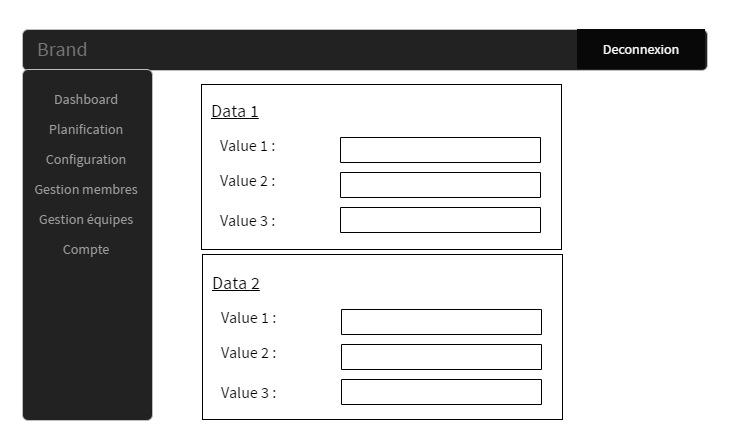
\includegraphics[scale=0.74]{figures/prototypes/Configuration.PNG}
  \caption{Prototype de la gestion des objectifs ICP}
  \label{code14}
\end{figure}
La figure \ref{code15} présente le prototype de l'interface de gestion d'équipe où l'utilisateur peut ajouter, modifier ou supprimer une équipe.
\begin{figure}[H]
  \centering
  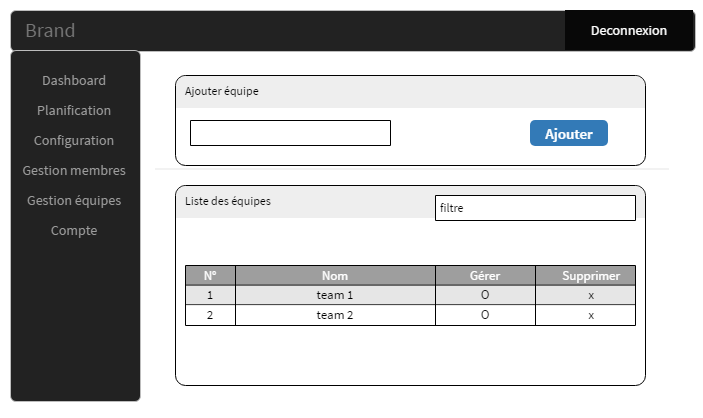
\includegraphics[scale=0.77]{figures/prototypes/Gestion_equipes_1.png}
  \caption{Prototype de la gestion des équipes}
  \label{code15}
\end{figure}
La figure \ref{code16} présente le prototype de l'interface de modification d'équipe où l'utilisateur peut changer le chef d'équipe ou enlever un utilisateur de cette dernière.
\begin{figure}[H]
  \centering
  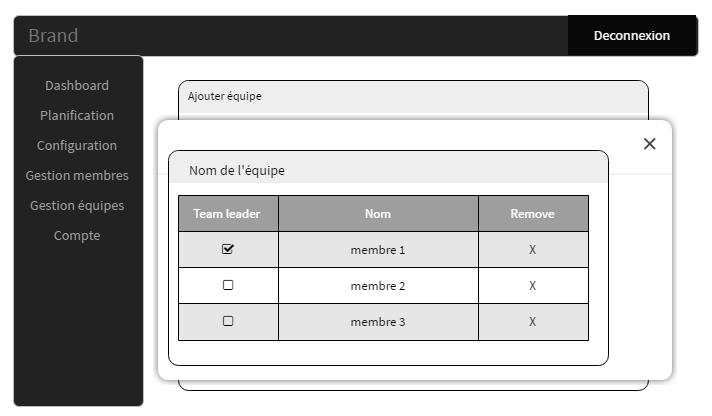
\includegraphics[scale=0.77]{figures/prototypes/Gestion_equipes_2.png}
  \caption{Prototype de la modification d'une équipe}
  \label{code16}
\end{figure}
La figure \ref{code17} présente le prototype de l'interface de gestion des membres où l'utilisateur peut ajouter, modifier ou supprimer un utilisateur de l'application.
\begin{figure}[H]
  \centering
  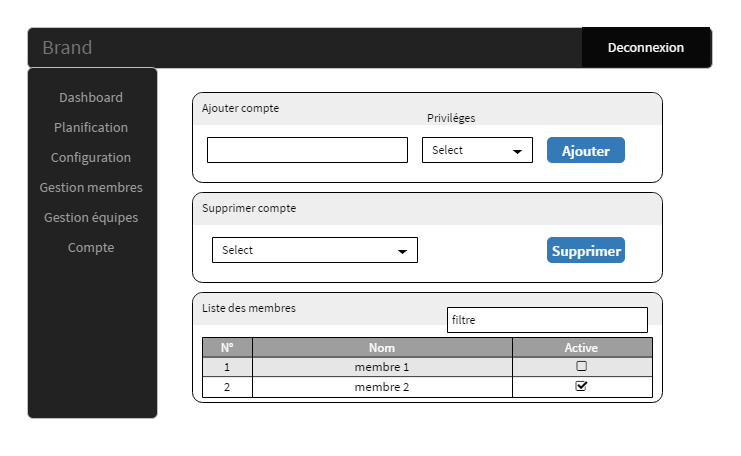
\includegraphics[scale=0.74]{figures/prototypes/Gestion_membres.PNG}
  \caption{Prototype de la gestion des membres}
  \label{code17}
\end{figure}
La figure \ref{code18} présente le prototype de l'interface de planification de tâche.
\begin{figure}[H]
  \centering
  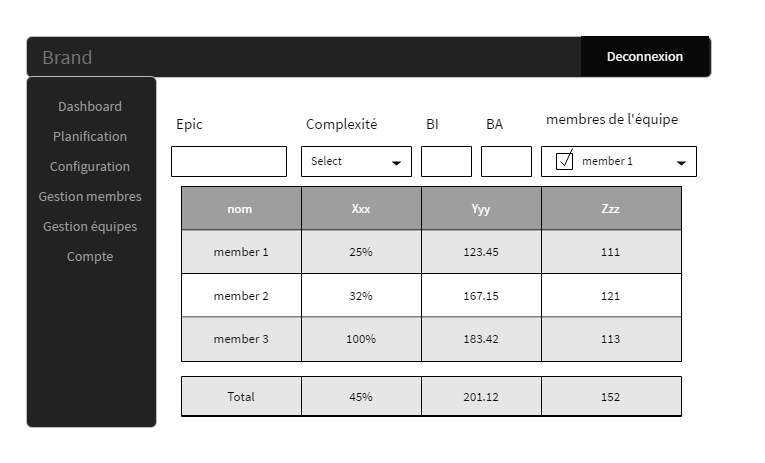
\includegraphics[scale=0.74]{figures/prototypes/Planification.PNG}
  \caption{Prototype de la planification}
  \label{code18}
\end{figure}

\section{Planification de release}
La planification de release est conçu pour décomposer le projet en plusieurs sprints de durée fixe. Pour pouvoir le faire, il faut estimer la complexité totale de user stories qui peuvent être réalisés dans une durée fixe du sprint. Cette valeur estimée s'appelle la vélocité \cite{Planning_sprint} \cite{Estimation_planification_Agile}. La durée d'un sprint pour notre projet va être fixé à 4 semaines et nous avons conclu que la vélocité sera égale à 21. La figure \ref{code19} représente la planification de release pour notre projet.

\begin{figure}[H]
\centering
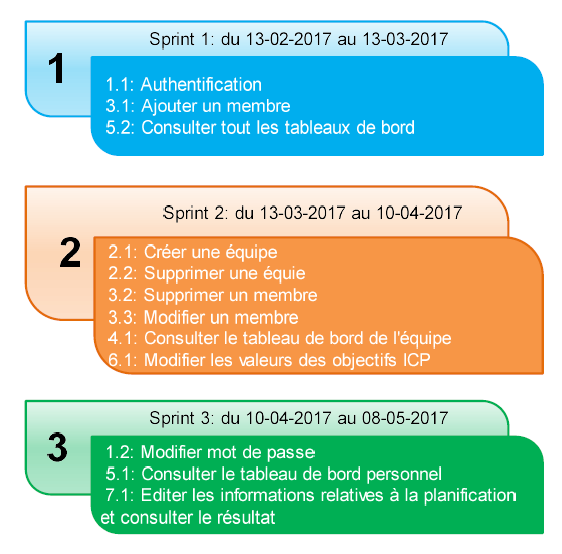
\includegraphics[scale=0.9]{figures/sprints_release_planification.png}
\caption{Planification de release de notre projet}
\label{code19}
\end{figure}
\section{Conclusion}
Dans ce chapitre nous avons présenté les besoins fonctionnels, les besoins non fonctionnels et les acteurs de notre application. Puis, nous avons présenté le diagramme de cas d'utilisation initiale. Après, nous avons défini la notion de priorité et celle de complexité. Ensuite, nous avons présenté le product backlog. Et enfin, nous avons présenté le prototypage et la planification de release qu'on va suivre tout au long de notre projet. Dans le prochain chapitre nous allons détailler nos choix architecturaux ainsi que l'environnement de travail matériel et logiciel.